\section{Cardinalità finite}
Ora inizia una breve carrellata fra le cardinalità più facile da definire. Parliamo qui di cardinalità finite, poi introdurremo la cardinalità numerabile e la cardinalità del continuo.

\begin{definition}[Insieme finito/infinito]
	Diciamo che $A$ è \vocab{finito} se $\exists n \in \omega \, |A| = |n|$. Se $A$ non è finito, diciamo che $A$ è \vocab{infinito}.
\end{definition}

Storicamente, è riflessiva una definizione alternativa di finitezza, data originariamente da Dedekind.

\begin{definition}[Dedekind-finitezza]
	Diciamo che $A$ è \vocab{Dedekind-finito} se non può essere messo in corrispondenza biunivoca con un suo sottoinsieme proprio. Ossia $A$ è Dedekind-finito se:
	\[ \forall B \subsetneq A \, |B| < |A|
		\]
\end{definition}

\subsection{Principio dei cassetti}
Con gli assiomi introdotti fino ad ora, possiamo solo dimostrare che finito $\rightarrow$ Dedekind-finito, mentre l'implicazione inversa è conseguenza dell'assioma della scelta.

\begin{proposition}[Principio dei cassetti - ossia finito $\rightarrow$ Dedekind-finito]
	\label{cassetti}
	Dato $A$ finito e $B$ un sottoinsieme proprio di $A$, $B \subsetneq A$, vale $|B| < |A|$. 
\end{proposition}

\begin{proof}
	Naturalmente $|B| \leq |A|$ vale perché l'identità $\id_B$ è una funzione iniettiva $B \rightarrow A$. Occorre quindi dimostrare che $|B| \ne |A|$.\\
	Per ipotesi $|A| = |n|$, per qualche $n \in \omega$, sia $g : A \to n$ una bigezione, si ha naturalmente che $|B| = |g[B]|$, e $g[B] \subsetneq n$, se verifichiamo che $|g[B]| < |n|$,
	allora otteniamo in automatico che $|B| < |A|$. Per fare ciò verifichiamo la disuguaglianza stretta nel caso in cui appunto l'insieme di partenza sia un naturale, dimostriamo per induzione la contronominale di questo fatto,
	ovvero dimostriamo che ogni sottoinsieme di un naturale con la sua stessa cardinalità è proprio il naturale stesso\footnote{La cui contronominale è appunto che ogni sottoinsieme proprio di $n$ ha cardinalità minore strettamente di quest'ultimo.}.
	\[ \textcolor{purple}{\forall n \in \omega \; \forall B \subseteq n (|B|=|n|\rightarrow B = n)}
		\]
	\begin{itemize}
		\item[$\boxed{\text{caso $n = \emptyset$}}$] Vera a vuoto perché $\emptyset$ non ha sottoinsiemi.
		\item[$\boxed{\text{caso $n = m + 1$}}$] Assumiamo per ipotesi induttiva che $\forall B \subseteq m (|B| = |m| \rightarrow B = m)$, vogliamo dimostrare che $\forall C \subseteq m + 1 (|C| = |m + 1| \rightarrow C = m + 1)$.\\
		Sia $f : m + 1 \rightarrow C$ una bigezione tra $m + 1$ e $C$, possiamo assumere, WLOG - vedremo alla fine perché -, che $f(m) = m$ (cioè che $m \in C$ e che è un punto fisso di $f$), in tal modo $f_{|m}$ sarà una bigezione tra $m$ e $C \setminus\{m\}$ (che è un suo sottoinsieme), per ipotesi induttiva ciò implica che $C \setminus \{m\} = m$,
		per cui $C \overset{\text{$f$ bigez.}}{=}\Imm(f) = m \cup \{f(m)\} = m \cup \{m\} = m + 1$.
		\begin{figure}[H]
			\centering
			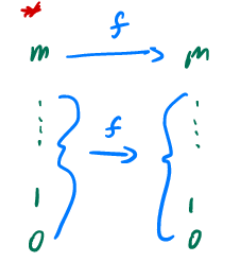
\includegraphics[width = 1.95cm]{immagini/cassetti1.png}
		\end{figure}
		Se $f(m) \ne m$ vediamo in primis che esiste sempre $a < m$ tale che $f(a) < m$ e inoltre possiamo sempre costruire una bigezione $f'$, a partire da $f$, tale per cui $f'(m) = m$.
		Se non esistesse $a < m$ tale per cui $f(a) = m$, allora $f_{|m}$ sarebbe una bigezione tra $m$ e $C \setminus\{f(m)\} \subseteq m$, che per ipotesi induttiva significa $C \setminus\{f(m)\} = m$,
		per cui $m \cup \{f(m)\} = m + 1 \implies f(m) = m$, contro l'assunto iniziale, per cui assurdo. Abbiamo ora che esiste $a < m$ tale per cui $f(a) = m$, quindi possiamo definire una nuova bigezione $f'$,
		che ha $m$ come punto fisso, nella maniera seguente:
		\[ f'(x) = \begin{cases}
			m &\text{se $x = m$} \\
			f(m) &\text{se $x = a$} \\
			f(x) &\text{altrimenti} \\
		\end{cases}
			\]
			\begin{figure}[H]
				\centering
				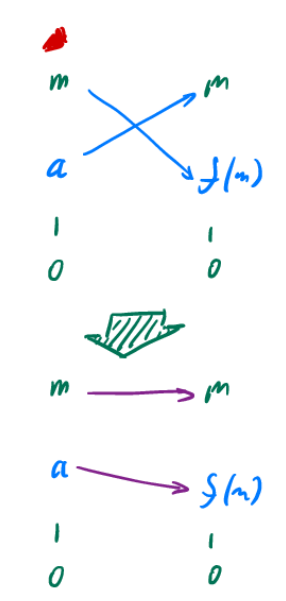
\includegraphics[width = 1.95cm]{immagini/cassetti2.png}
			\end{figure}
	\end{itemize}
\end{proof}

\begin{corollary}[$A$ finito $\implies$ ha un'unica cardinalità]
	Se $A$ è un insieme finito, allora esiste ed è unico un elemento di $\omega$ con cui è in bigezione:
	\[ \exists \textcolor{red}{!} n \in \omega \; |A| = |n|
		\]
\end{corollary}

\begin{proof}
	Se $|m| = |A| = |n|$, possiamo assumere, senza perdita di generalità $m \leq n$, che corrisponde a $m \subseteq n$, quindi per il \hyperref[cassetti]{principio dei cassetti} $m = n$.
\end{proof}

Se adesso volessimo dimostrare il viceversa: [che formulato in versione contronominale è] che un insieme infinito non è Dedekind-finito, quale sarebbe l'ostacolo? Abbiamo già osservato che $\omega$ non è finito, perché la funzione successore 
stabilisce una corrispondenza biunivoca fra $\omega$ e $\omega \setminus\{0\} \subsetneq \omega$ (quindi non è Dedekind-finito, e per la contronominale del \hyperref[cassetti]{principio dei cassetti} non è finito). Ne segue la seguente osservazione.

\begin{remark}
	\label{omega_Dedekind_finito}
	Se esiste $f : \omega \rightarrow A$ iniettiva, allora $A$ non è Dedekind-finito.\footnote{E quindi in automatico non è finito.}
\end{remark}

\begin{proof}
	Basta considerare la funzione iniettiva:
	\[ g : A \to A : a \mapsto \begin{cases}
		f \circ s \circ f^{-1}(a) &\text{se $a \in f[\omega]$} \\
		\id_A(a) &\text{altrimenti}
	\end{cases}
		\]
	È immediato vedere che $\Imm(g) = A \setminus \{f(0)\} \subsetneq A$ (l'unico escluso è lo 0, perché non può esserci un elemento che ha come controimmagine un elemento di $\omega$ il cui
	successore sia 0, perché per quanto visto non esiste), dunque $A \hookrightarrow \Imm(g) \subsetneq A$, pertanto è in bigezione con un suo sottoinsieme proprio, per cui non può essere Dedekind-finito.\footnote{È l'argomento dell'\href{https://en.wikipedia.org/wiki/Hilbert\%27s_paradox_of_the_Grand_Hotel}{\textcolor{purple}{hotel di Hilbert}}.}
	\begin{figure}[H]
		\centering
		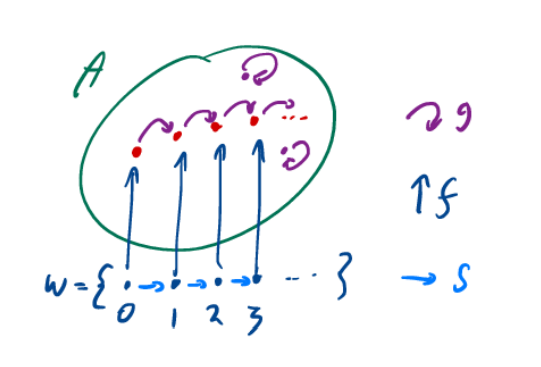
\includegraphics[width = 4.5cm]{immagini/cassetti3.png}
	\end{figure}
\end{proof}

Quindi ci basterebbe dimostrare che $\omega$ si immerge in ogni insieme infinito (e dal lemma appena visto avremmo che l'insieme non è Dedekind-finito, completando l'altra freccia del principio dei cassetti).
Un tentativo di dimostrazione potrebbe andare come segue.

\begin{proof}
	Sia $A$ infinito, costruiamo per ricorsione, seconda forma, una $f : \omega \rightarrow A$ iniettiva. Supponiamo di conoscere $f_{|n}$, il nostro scopo è definire il prossimo valore: $f(n)$.
	Siccome $A$ è infinito, $f_{|n}$, che è iniettiva per costruzione, non può essere surgettiva, quindi esiste $a \in A$ con $a \not \in \Imm(f_{|n})$. Pongo $f(n) = a$.
\end{proof}

Dov'è l'errore? Nell'ultima riga! Noi sappiamo che, data $f_{|n}$, esistono degli $a \in A$ con $a \not\in\Imm(f_{|n})$, questo è corretto. È anche corretto che ci basterebbe porre $f(n) =$``uno qualunque di questi $a$''.
Il guaio è che, \textcolor{MidnightBlue}{per applicare il teorema di ricorsione}, ci serve una funzione che fissa uno degli $a$ da poter usare come $h$ del teorema di ricorsione (più precisamente, vorremmo definire $h$ come un elemento di $A \setminus \Imm(f_{|n}) \ne \emptyset$, poiché tuttavia dobbiamo ripetere questo procedimento infinite volte - per ogni $n \in \omega$ -,
non possiamo fissare infiniti elementi tutti assieme - che è equivalente allo scrivere $h$ come insieme quale è - con gli assiomi attualmente a disposizione, infatti possiamo per ora fissare soltanto un numero finito di cose).
A patto di averne una, ne andrebbe bene una qualunque.\\ Purtroppo però, a partire dalla mera ipotesi che $A$ è infinito, non abbiamo modo di procurarci nessuna funzione del genere. Potremmo cavarcela se avessimo qualche struttura su $A$, sulla quale far leva - per esempio per dire ``prendo il minimo 
fra gli $a \not\in \Imm(f_{|n})$'', o ``prendo il più giallo'' - ma di $A$ non sappiamo nulla, e non abbiamo modo di indurre una struttura di questo genere.\\
Accettato che non possiamo dimostrare che $\omega$ si immerge in qualsiasi insieme infinito, possiamo però lambire questa soglia: dimostriamo che, in un insieme infinito, si immergono tutti i numeri naturali.

\begin{proposition}[Tutti i naturali si immergono in un qualsiasi insieme infinito]
	Sia $A$ infinito, allora $\forall n\in \omega \; |n| < |A|$.
\end{proposition}

\begin{proof}
	Basta dimostrare il $\leq$, infatti $|n| < |n+1| \leq |A|$. Dimostriamo per induzione su $n$ che c'è una funzione iniettiva da $n$ ad $A$.
	\begin{itemize}
		\item[$\boxed{\text{caso $n = 0$}}$] La funzione vuota, $f = \emptyset$ che va dal vuoto a qualsiasi insieme, va bene.
		\item[$\boxed{\text{caso $n = m+1$}}$] Per ipotesi induttiva esiste $f : m \rightarrow A$ iniettiva. Siccome $A$ è infinito (e $m$ è finito), $A \setminus \Imm(f) \ne \emptyset$, quindi esiste $a \in A \setminus \Imm(f)$ e possiamo prenderlo (stiamo fissando una sola cose e possiamo farlo).
		Definiamo la funzione $f' = f \cup \{(n,a)\}$, che è iniettiva in quanto unione di funzioni iniettive su insiemi disgiunti - in arrivo.
	\end{itemize}
\end{proof}

\begin{corollary}[Ovvietà]
	Un sottoinsieme di un insieme finito è finito.
\end{corollary}

\begin{proof}
	Sia $A$ finito e $B \subseteq A$. Se, per assurdo $B$ fosse infinito, avremmo:
	\[ |B| \overset{B \subseteq A}{\leq} |A| \overset{\text{$A$ finito}}{=} |n| \overset{\text{prop. sopra}}{<} |B| \;\textcolor{red}{\lightning}
		\]	
\end{proof}

\begin{exercise}
	\label{disuguaglianze_senza_AC1}
	Dimostrare che:
	\begin{itemize}
		\item se $|A| < |n|$ con $n \in \omega$, allora $|A| = |m|$ per qualche $m < n$.
		\item se $A$ è finito e $f : A \rightarrow B$, allora $f[A]$ è finito.
	\end{itemize}	
\end{exercise}

\begin{soln}
	Verifichiamo le due cose separatamente.
	\begin{itemize}
		\item Per ipotesi esiste $f : A \to n$ iniettiva e non surgettiva, abbiamo quindi $f[A] \subseteq n$, e per il corollario sopra un sottoinsieme di un insieme finito è finito, ovvero $\exists m \in \omega \; |f[A]| = m$.
		Osserviamo che necessariamente $m < n$, se fosse $m \geq n$, per la definizione di ordinamento su $\omega$, ciò corrisponde a $m \supseteq n \implies |m| \geq |n|$, per cui:
		\[ |A| \overset{\text{$f$ iniett.}}{=} |f[A]| = |m| \geq |n| \overset{\text{Hp.}}{>} |A| \;\textcolor{red}{\lightning}
			\] 
		\item Se verifichiamo che $|f[A]| \leq |A|$, essendo $A$ finito, otteniamo $|f[A]| \leq |n|$, per qualche $n \in \omega$, e, o $|f[A]| = |n|$, oppure $|f[A]| < |n|$ e quindi vale il punto precedente, in ogni caso si ottiene $f[A]$ finito.\\
		Ci resta da verificare l'assunzione iniziale, possiamo farlo sfruttando il buon ordinamento di $\omega$ tramite la seguente funzione:
		\[ g : f[A] \to A : x \mapsto h^{-1}\left(\min_{<_{|n}}(h[f^{-1}(x)])\right)
			\]
		dove $<_{|n}$ è l'ordine usuale di $\omega$ ristretto ad $n$ e $h$ è la bigezione che esiste per ipotesi da $A$ ad $n$.
		Si vede facilmente che $g$ è ben definita, verifichiamo che è anche iniettiva:
		\[	\begin{split}
			g(x) = g(y) &\iff h^{-1}\left(\min_{<_{|n}}\{h[f^{-1}(x)]\}\right) = h^{-1}\left(\min_{<_{|n}}\{h[f^{-1}(y)]\}\right) \\
						&\iff \min_{<_{|n}}\{h[f^{-1}(x)]\} = \min_{<_{|n}}\{h[f^{-1}(y)]\} \\
						&\iff h(a) = h(b)
		\end{split}
			\]
		con $a \in f^{-1}(x)$ e $b \in f^{-1}(y)$ (in altre parole abbiamo dato un nome ai minimi). Ora, essendo $h$ bigettive quanto scritto equivale ad $a  = b$, che, applicando $f$,
		equivale a:
		\[ x = f(a) \overset{a = b}{=} f(b) = y
			\]
		per cui $g$ è iniettiva e vale la disuguaglianza iniziale.
	\end{itemize}
\end{soln}

\subsection{Operazioni fra le cardinalità finite}

\begin{proposition}[Corrispondenza tra le operazioni su $\omega$ e quelle tra cardinalità finite]
	\label{op_card_fin}
	Dati $m,n \in \omega$ vale che:
	\[ |m| + |n| = |m+n| \qquad |m|\cdot|n| = |m \cdot n| \qquad |m|^{|n|} = |m^n|
		\]
	ovvero, per gli elementi di $\omega$ le operazioni tra cardinalità corrispondo alla cardinalità delle operazioni tra gli elementi, già definite per ricorsione su $\omega$.
\end{proposition}

\begin{proof}
	Dimostriamo, intanto che $|m| + |1| = |s(m)|$. A sinistra abbiamo, infatti la cardinalità di $(m \times \{0\}) \cup \{(0,1)\}$\footnote{Typo di Mamino sui suoi appunti in quanto $1 = \{0\}$.} e a destra abbiamo la cardinalità di $m \cup \{m\}$.
	Quest'ultimo insieme si mappa bigettivamente nel primo, mandando $x \in m$ in $(x,0)$ e $m$ in $(0,1)$. 
	Ora, le uguaglianze asserite seguono, per induzione su $n$, dalle proprietà delle operazioni sulle cardinalità e dalla definizione ricorsiva delle operazioni su $\omega$.\\
	\textcolor{purple}{$|m|+|n| = |m+n|$}
	\begin{itemize}
		\item[$\boxed{\text{caso $n = 0$}}$] $|m| + |0| =  |(m \times \{0\}) \cup \emptyset| = |m| = |m + 0|$.
		\item[$\boxed{\text{caso $n = s(a)$}}$] Per ipotesi induttiva abbiamo $|m| + |a| = |m + a|$, da cui possiamo verificare la tesi come segue:
		\begin{align*}
			|m| + |s(a)| \overset{\text{oss. iniziale}}{=}\quad& |m| + (|a| + |1|) \\
						 \overset{\text{propr. operaz. card.}}{=}& (|m| + |a|) + |1| \\
						 \overset{\text{Hp. indutt}}{=}\quad& |m+a| + |1| \\
						 \overset{\text{oss. iniziale}}{=}\quad& |s(m+a)| \\
						 \overset{\text{def. di $+$}}{=}\quad\;& |m + s(a)|
 		\end{align*}
	\end{itemize}
	\textcolor{purple}{$|m|\cdot|n| = |m \cdot n|$}
	\begin{itemize}
		\item[$\boxed{\text{caso $n = 0$}}$] $|m| \cdot |0| =  |m \times \emptyset| = |0| \overset{\text{def. di $\cdot$}}{=} |m \cdot 0|$.
		\item[$\boxed{\text{caso $n = s(a)$}}$] Per ipotesi induttiva abbiamo $|m|\cdot|a| = |m \cdot a|$, da cui possiamo verificare la tesi come segue:
		\[ \begin{split}
			|m| \cdot |s(a)| \overset{\text{oss. iniziale}}{=}\quad& |m| \cdot (|a| + |1|) \\
						 \overset{\text{propr. operaz. card.}}{=}& |m| \cdot |a| + \underbrace{|m| \cdot |1|}_{|m \times \{0\}| = |m|} \\
						 \overset{\text{Hp. indutt}}{=}\quad& |m \cdot a| + |m| \\
						 \overset{\text{propr. $+$ card. fin.}}{=}\quad& |m \cdot a + m| \\
						 \overset{\text{def. di $\cdot$}}{=}\quad\;& |m \cdot s(a)|
 		\end{split} 
			\]
	\end{itemize}
	\textcolor{purple}{$|m|^{|n|} = |m^n|$}
	\begin{itemize}
		\item[$\boxed{\text{caso $n = 0$}}$] $|m|^{|0|} =  |{}^{0}m| = |\{f : 0 \rightarrow m\}| = |\{\emptyset\}| =  |1| = |m^0|$ (l'unica funzione possibile dal vuoto a $m$ è $f = \emptyset$\footnote{E quindi ${}^0m = \{f : \emptyset \rightarrow m\} = \{\emptyset\} = 1$, o in alternativa si può pensare che
		$f \subseteq \emptyset \times m = \emptyset \implies f \in \ps(\emptyset) = \{\emptyset\}$ e quindi $f = \emptyset \implies {}^0m = \{f\} = \{\emptyset\} = 1$.}).
		\item[$\boxed{\text{caso $n = s(a)$}}$] Per ipotesi induttiva abbiamo $|m|^{|a|} = |m^a|$, per cui abbiamo:
		\[ \begin{split}
			|m|^{|s(a)|} \overset{\text{oss. iniziale}}{=}\quad& |m|^{|a| + |1|} \\
						 \overset{\text{propr. operaz. card.}}{=}& |m|^{|a|} \cdot |m|^{|1|} \textcolor{MidnightBlue}{= |m| }\\
						 \overset{\text{Hp. indutt}}{=}\quad& |m^a| \cdot |m| \\
						 \overset{\text{caso prec.}}{=}\quad& |m^a \cdot m| \\
						 \overset{\text{def. potenza}}{=}\quad\;& |m^{s(a)}|
 		\end{split} 
			\]
		(dove $|m|^{|1|} = |m|$ perché $|{}^{1}m|  = |\{f : 1 \rightarrow m\}| = |\{\{(0,0)\},\{(0,1)\},\{(0,2)\},\ldots,\linebreak(0,m-1)\}|$, e quest'ultimo insieme è banalmente in bigezione con $m$).
	\end{itemize}
\end{proof}

\begin{note}
	Questa proposizione ci fornisce una dimostrazione delle proprietà aritmetiche elementari delle operazioni su $\omega$ [sfruttando le proprietà delle operazione fra cardinalità], alternativa a quella per induzione (che è stata lasciata per esercizio).
	Basta, infatti, applicare le corrispondenti proprietà delle operazioni sulle cardinalità\footnote{E ciò non comporta problemi di circolarità poiché nella dimostrazione della proposizione precedente abbiamo usato \textbf{solo} la definizione delle tre operazione e nessuna delle  loro proprietà.}.
\end{note}

\begin{exercise}
	Dimostra che se $m,n \in \omega$ e $m \leq n$, esiste un unico $n-m \in \omega$ tale che $m + (n-m) = n$. In due modi diversi.
\end{exercise}

I due modi sono sostanzialmente l'induzione ed il principio del minimo (idea la quale sarà riutilizzata in maniera molto simile per dimostrare il lemma di sottrazione ordinale), partiamo da quest'ultimo modo.

\begin{soln}
	Fissati $m,n \in \omega$, con $m \leq n$, dobbiamo verificare esistenza ed unicità di $k \in \omega$ tale che $m + k = n$.
	\begin{itemize}
		\item[$\boxed{\text{unicità}}$] Per l'unicità ci basta osservare che la funzione somma è strettamente crescente in entrambe le componenti\footnote{Andrebbe verificato per induzione.}, dunque qualsiasi $k' \ne k$, per l'ordinamento totale di $\omega$, è necessariamente strettamente maggiore o minore di $k$, da cui la somma con $m$ è a sua volta strettamente maggiore o minore di $n$.
		\item[$\boxed{\text{esistenza}}$] Se $m = n$, allora $k = 0$ e si conclude. Possiamo quindi supporre che $m < n$, sia $d$ il minimo tale per cui $m + d > n$, tale minimo esiste perché $n < s(n) < m + s(n)$, dunque l'insieme in cui è preso è non vuoto e bene ordinato, pertanto $d$ è ben definito. Poiché $m < n$ si ha $d > 0$, dunque $d = b + 1$, e per la minimalità
		di $d$ si ha $m + b \leq n$, dove in particolare, se valesse il $<$, si avrebbe $m + d = m + s(b) = s(m + b) \leq n$, che è assurdo, dunque vale l'uguaglianza e $b$ è il $k$ cercato.
	\end{itemize}
\end{soln}

Vediamo ora la stessa cosa dimostrata facendo uso dell'induzione numerabile.

\begin{soln}
	Per l'unicità si procede esattamente come sopra, dimostriamo per induzione (su $n$) che fissati $m,n \in \omega$, con $m \leq n$, esiste $k \in \omega$ tale che $m + k = n$.
	\begin{itemize}
		\item[$\boxed{\text{caso $n = 0$}}$] In tal caso, o $m < n = 0$, e quindi la tesi è vera a vuoto, oppure $m = n = 0$, ed in questo caso basta prendere $k = 0$.
		\item[$\boxed{n \implies n + 1}$] Supponiamo che esista $k \in \omega$ tale che $m + k = n$ e verifichiamo che esista $k' \in \omega$ tale che $m + k' = n + 1$. Dall'ipotesi induttiva:
		\[ m + k = n \implies m + s(k) = s(m + k) = s(n) = n + 1
			\]
		per cui prendiamo proprio $k ' = k + 1$.
	\end{itemize}
\end{soln}